This section details the characterization of the SiPM S13360-1375 model, which was the first choosen as TRITIUM monitor photosensor. This characterization is incomplete since some important SiPM parameters for the TRITIUM monitor, which are PDE, dark count rate and crosstalk probability, were not measured. A complete characterization is already underway for the S13360-6075 model, the latest proposal for the TRITIUM detector, where the relevant parameters, given in section \ref{subsubsec:SiPM}, will be experimentaly determined using the experimental setup, described in appendix \ref{App:ElectronicReadoutSiPM}. The SiPM characterization is carried out inside of a climatic chamber, model CCM 81 from DYCOMETAL \cite{ClimaticChamberIFIMED}. This climatic chamber allows to control the temperature and humidity with a precisión of $0.1\celsius$ and $0.1\%$ respectively. In addition, this chamber is a Faraday cage. A special black blanket \cite{BlackBlancket} was used to prevent external photons from reaching the SiPM.

First, the quenching resistance and the breakdown voltage of the SiPM were obtained from the measurement of the current-voltage curves of the SiPM with the bias voltage applied in forward and reverse direction, respectively. This measurement was done without the amplification of the electronic board to achieve a better precision in the dark. The output current of the SiPM was directly measured using the Keithley 6487 Picoammeter/Voltage Source \cite{DataSheetKeithley6487}. The LabView sofware was used to take the data. The measured parameters are plotted as a function of the bias voltage in Figure \ref{fig:IVcurveSiPM}.

\begin{figure}
\centering
    \begin{subfigure}[b]{0.9\textwidth}
    \centering
    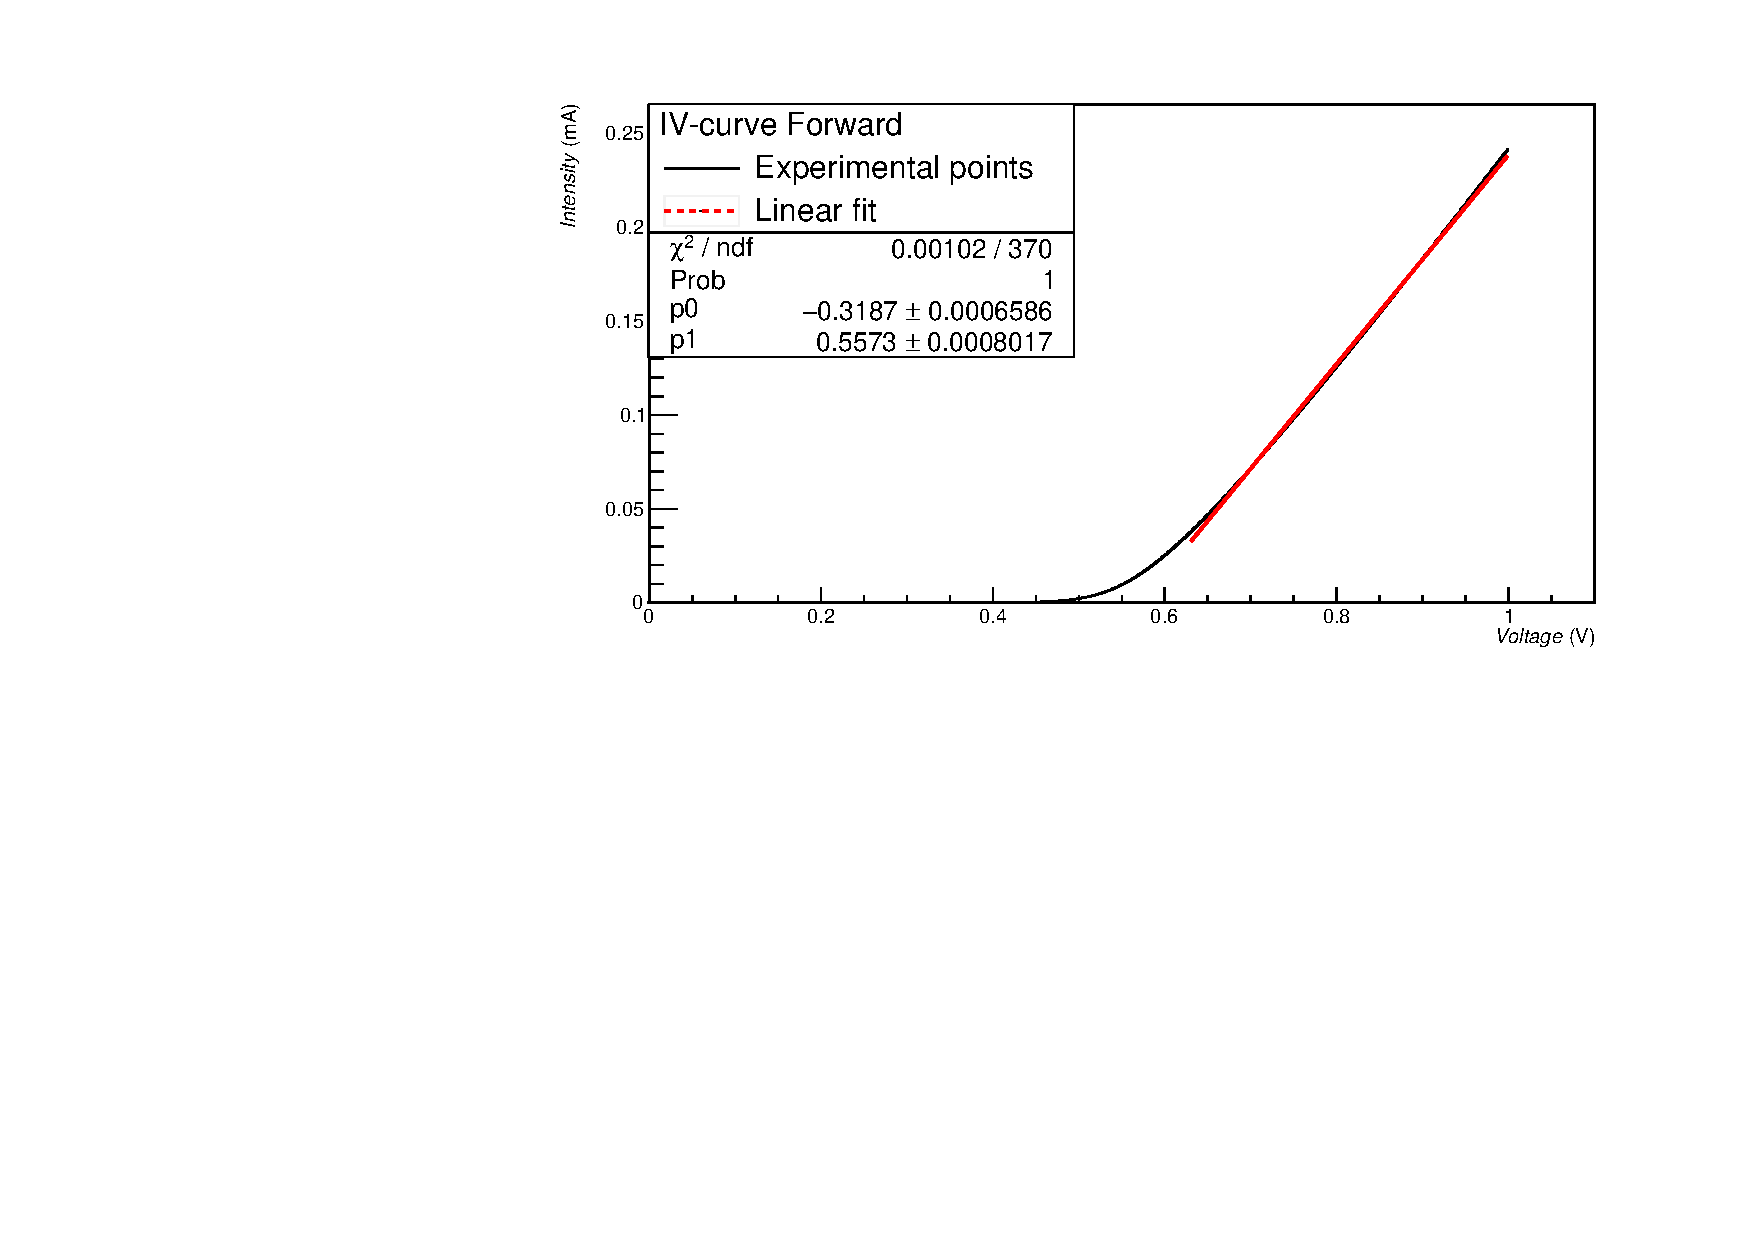
\includegraphics[width=\textwidth]{4ResearchAndDevelopments/42SiPM/IVCurveSiPMForward.pdf}  
    \caption{\label{subfig:IVcurveForward}}
    \end{subfigure}
    \hfill
    \begin{subfigure}[b]{0.9\textwidth}
    \centering
    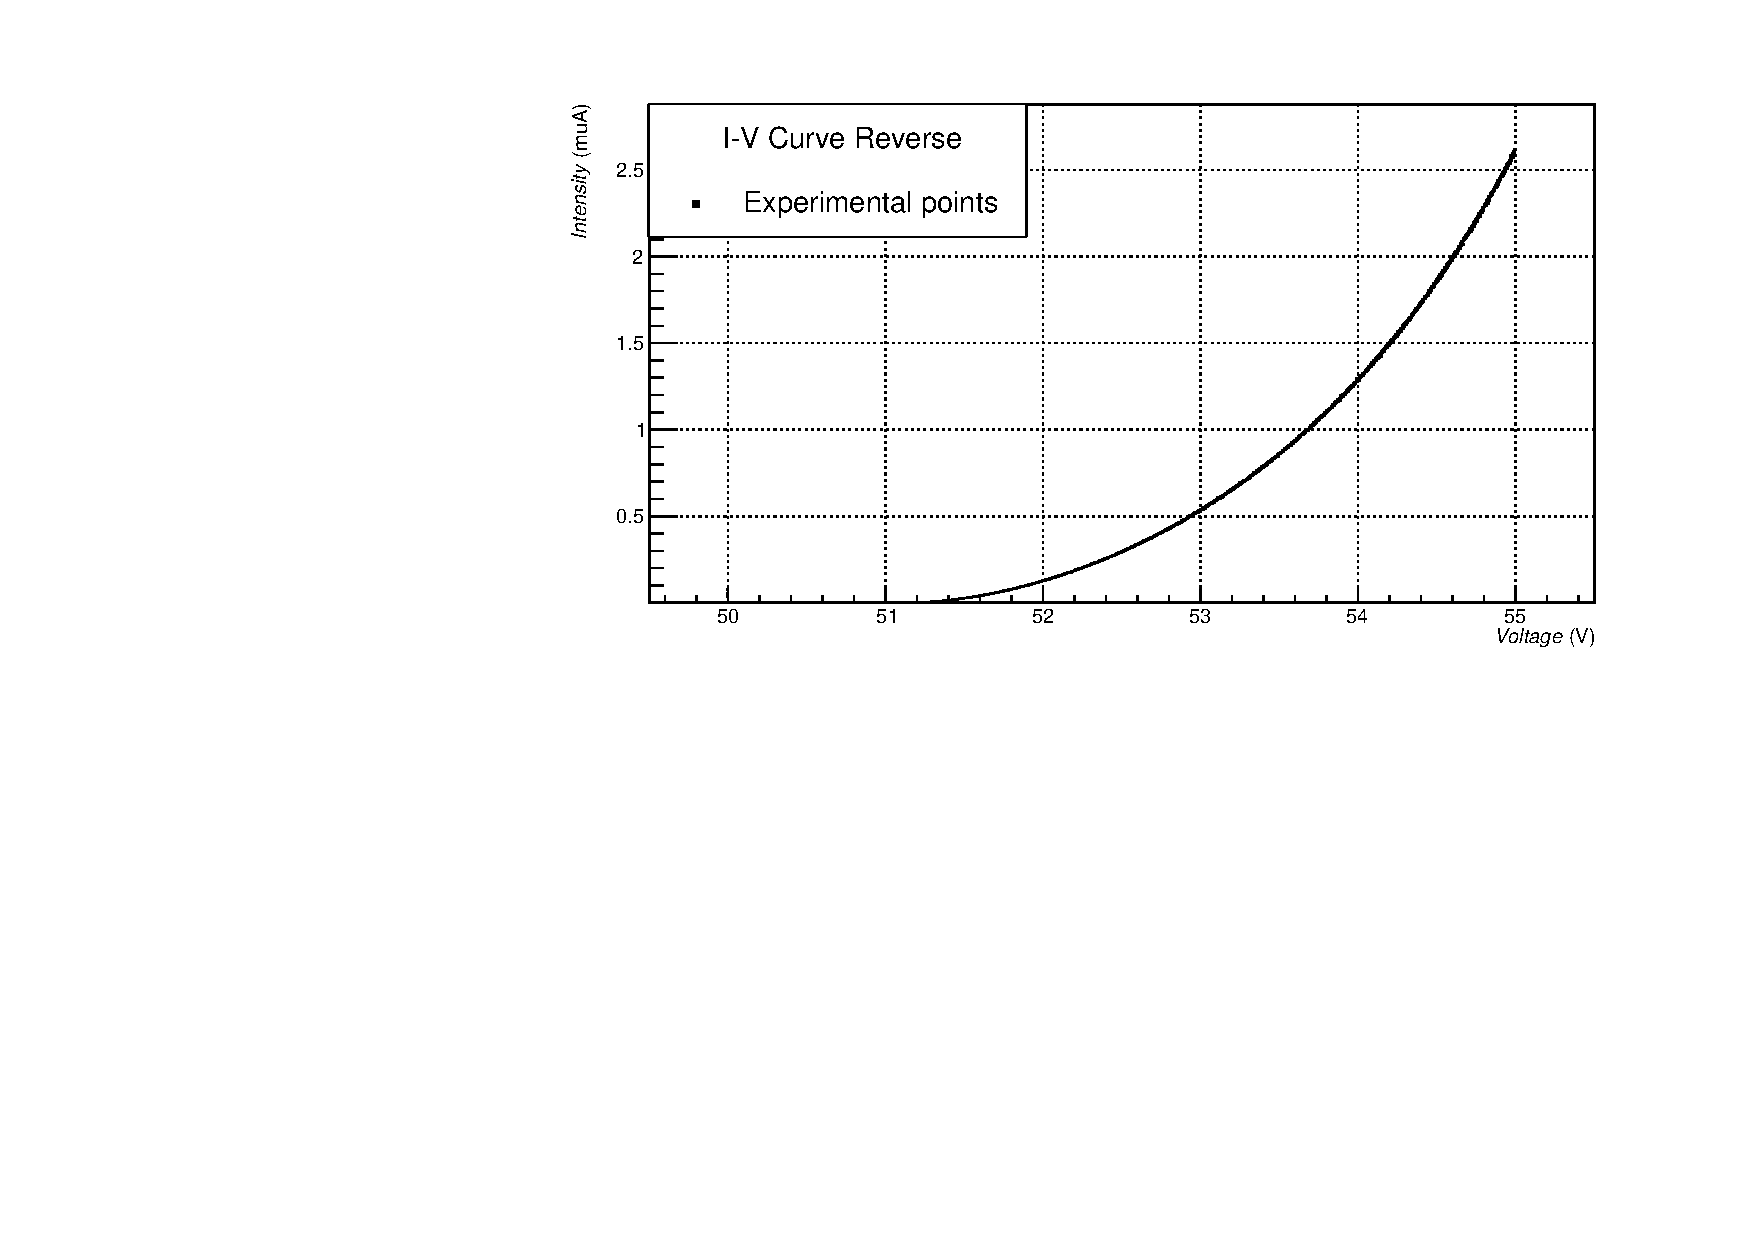
\includegraphics[width=\textwidth]{4ResearchAndDevelopments/42SiPM/IVCurveSiPMReverse.pdf}  
    \caption{\label{subfig:IVcurveReverse}}
    \end{subfigure}
 \caption{I-V curves measured for the SiPM S13360-1375 model with the bias voltage applied in a) forward direction b) reverse direction. Measurements taken at $T=25\celsius$ and humidity $H=45\%$.}
 \label{fig:IVcurveSiPM}
\end{figure}

As can be seen, when the bias voltage is applied in forward direction, Figure \ref{subfig:IVcurveForward}, the output current of the SiPM does not flow until the potential difference between the n and p layers is reached, which is approximately $V_0=0.7~\volt$ for silicon photosensors, close to the value experimentally obtained, $V_0= 0.5~\volt$. When the current start to flow, the intensity is linear with the applied voltage. The equivalent resistance, $R_{eq}$, was determined from, 
\begin{equation}
I=\frac{1}{R_{eq}}V;  \qquad \frac{1}{R_{eq}} = \sum_{i=1}^{N}\frac{1}{R_{qi}}= \frac{N}{R_{q}}
\label{QuenchingResistance}
\end{equation}
and $R_{iq}$ are the quenching resistance of each pixel of the SiPM in parallel which have the same value, $R_{q}$. A value of $R_{q}= 360.56 \pm 0.07~\kilo\ohm$ was obtained, which is in agreement with the typical values given by Hamamatsu.

The breakdown voltage, $V_{BD}$, was obtained from the reverse bias voltage plot. This is the points at which the output current of SiPM start to flow, which can be calculated from the maximum of the function 
\begin{equation}
f=\frac{1}{I}\frac{dI}{dV}
\label{BreakDownVoltageFunction}
\end{equation}

The value obtained, $V_{BD}=51.02~\volt$, is in agreement with the value provided by Hamamatsu, Table \ref{tab:PropertiesOfSiPM1375}.

To measure the SiPM gain, $G_{SiPM}$, the electronic board described in section \ref{subsubsec:SiPMsElectronicalSystem} with an amplification factor of $F_{amp}=170$ was used. An incoherent light source, LED435-03 from Toithner LaserTechnik Gmbh \cite{LEDRLT}, described in section \ref{subsec:CharacterizationFibers}, was used to illuminate the SiPM with a low enough flux of $\lambda= 435~\nm$ photons. The SiPM output signal shows various well-defined pulse heights, shown in Figure \ref{fig:OutputPulses_SPSspectrum}, corresponding to the number of pixels simultaneously fired. The single photon spectrum, SPS is plotted in Figure \ref{fig:OutputPulses_SPSspectrum}. This spectrum was obtained by integrating and hitogramming the SiPM output pulses with time windows wide enough to contain the full charge of the pulse. The time windows used in these measurements was $t_w= 500~\nano\second$. The light source gave a trigger signal for the measurement, green line in Fig \ref{fig:OutputPulses_SPSspectrum}.

\begin{figure}[hbtp]
\centering
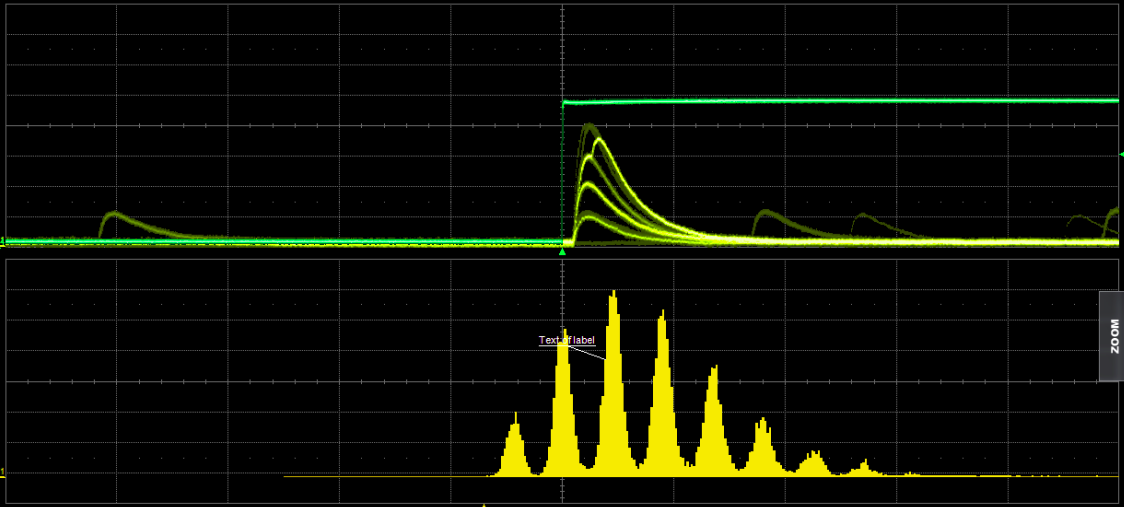
\includegraphics[scale=0.3]{4ResearchAndDevelopments/42SiPM/SiPMPulses_SPS_Spectrum.png}
\caption{Above) Trigger signal (green) and SiPM output pulses (yellow). Below) SPS spectrum obtained by integrating and histograming the SiPM output pulses. This measurement was done at $25\celsius$, $V_{bias}=53.98$ and humidity of $H=60\%$. \label{fig:OutputPulses_SPSspectrum}}
\end{figure}

The well-separated peaks in the SPS spectrum correspond to the charge produced by a different number of fired pixels. The first peak in the spectrum is the pedestal, which is the charge measured when no pixel is fired. This peak is caused by the electronic noise of the system. The second peak corresponds to one fired pixel and so on. The SiPM gain, $G_{SiPM}$, can be obtained from the SPS spectrum from the equation,
\begin{equation}
G=\frac{\overline{\Delta Q}(V \cdot{} s)}{F_{amp}(V/A) \times e^-(C)}
\label{SiPMGain}
\end{equation}
where $e^-$ is the electron charge and $\overline{\Delta Q}$ is the average peak distance in the SPS spectrum, corresponding to the charge released by a fired pixel. 

To obtain the value of $\overline{\Delta Q}$ a macro was written in ROOT \cite{ROOTWebPage}. This macro finds and extract the bakcground, which is crucial in some cases like high temperatures or high bias voltages. After that, this macro find all peaks in the SPS spectrum and fits each one to a Gaussian funtion, shown in Figure \ref{subfig:GaussianFitSiPMs}. The value and error of the charge produced by multiple fired pixels are obtained from the centroid and the sigma of the different fitted Gaussian functions. The obtained charges are fitted to the number of fired pixels, Figure \ref{subfig:LinearFitSiPMGain}.

\begin{figure}
\centering
    \begin{subfigure}[b]{0.47\textwidth}
    \centering
    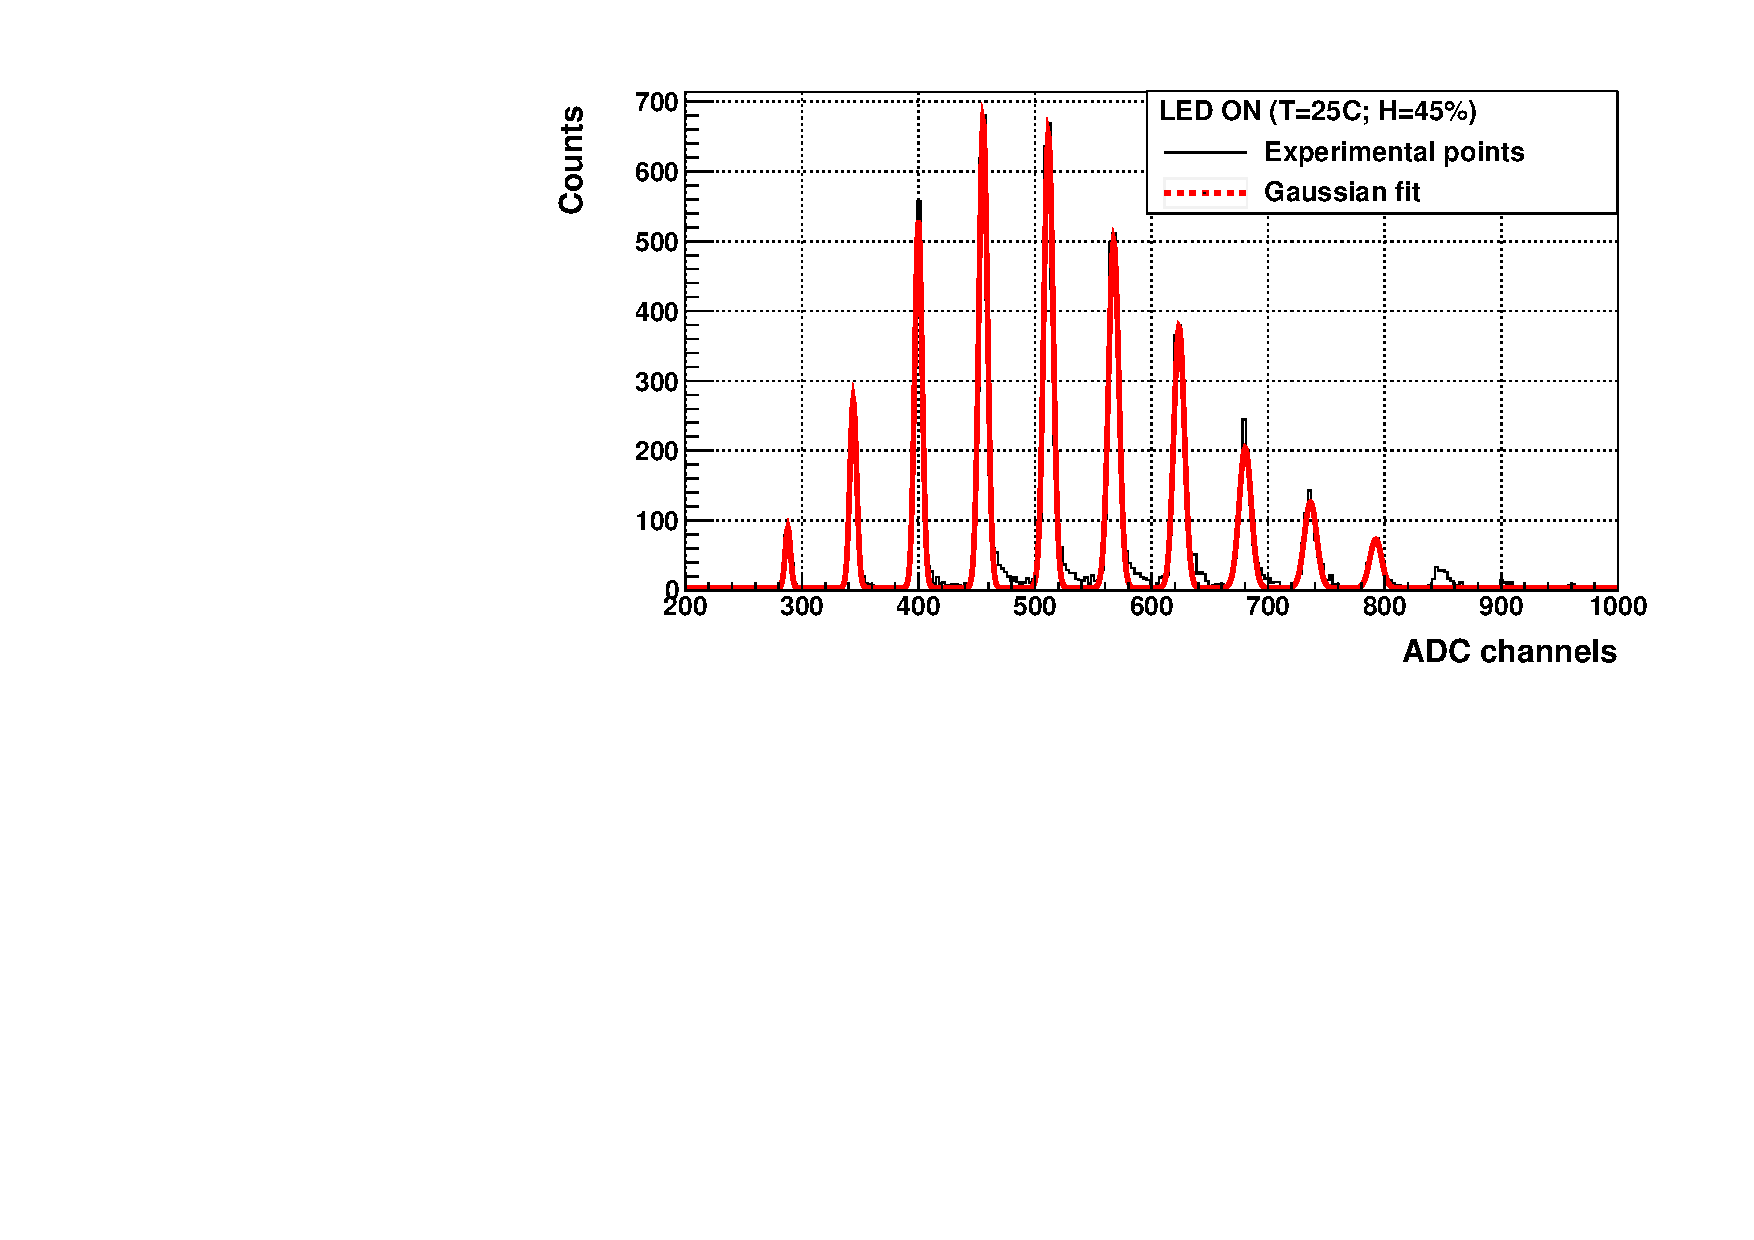
\includegraphics[width=\textwidth]{4ResearchAndDevelopments/42SiPM/GaussianFitSPSSpectrum.pdf}  
    \caption{\label{subfig:GaussianFitSiPMs}}
    \end{subfigure}
    \hfill
    \begin{subfigure}[b]{0.47\textwidth}
    \centering
    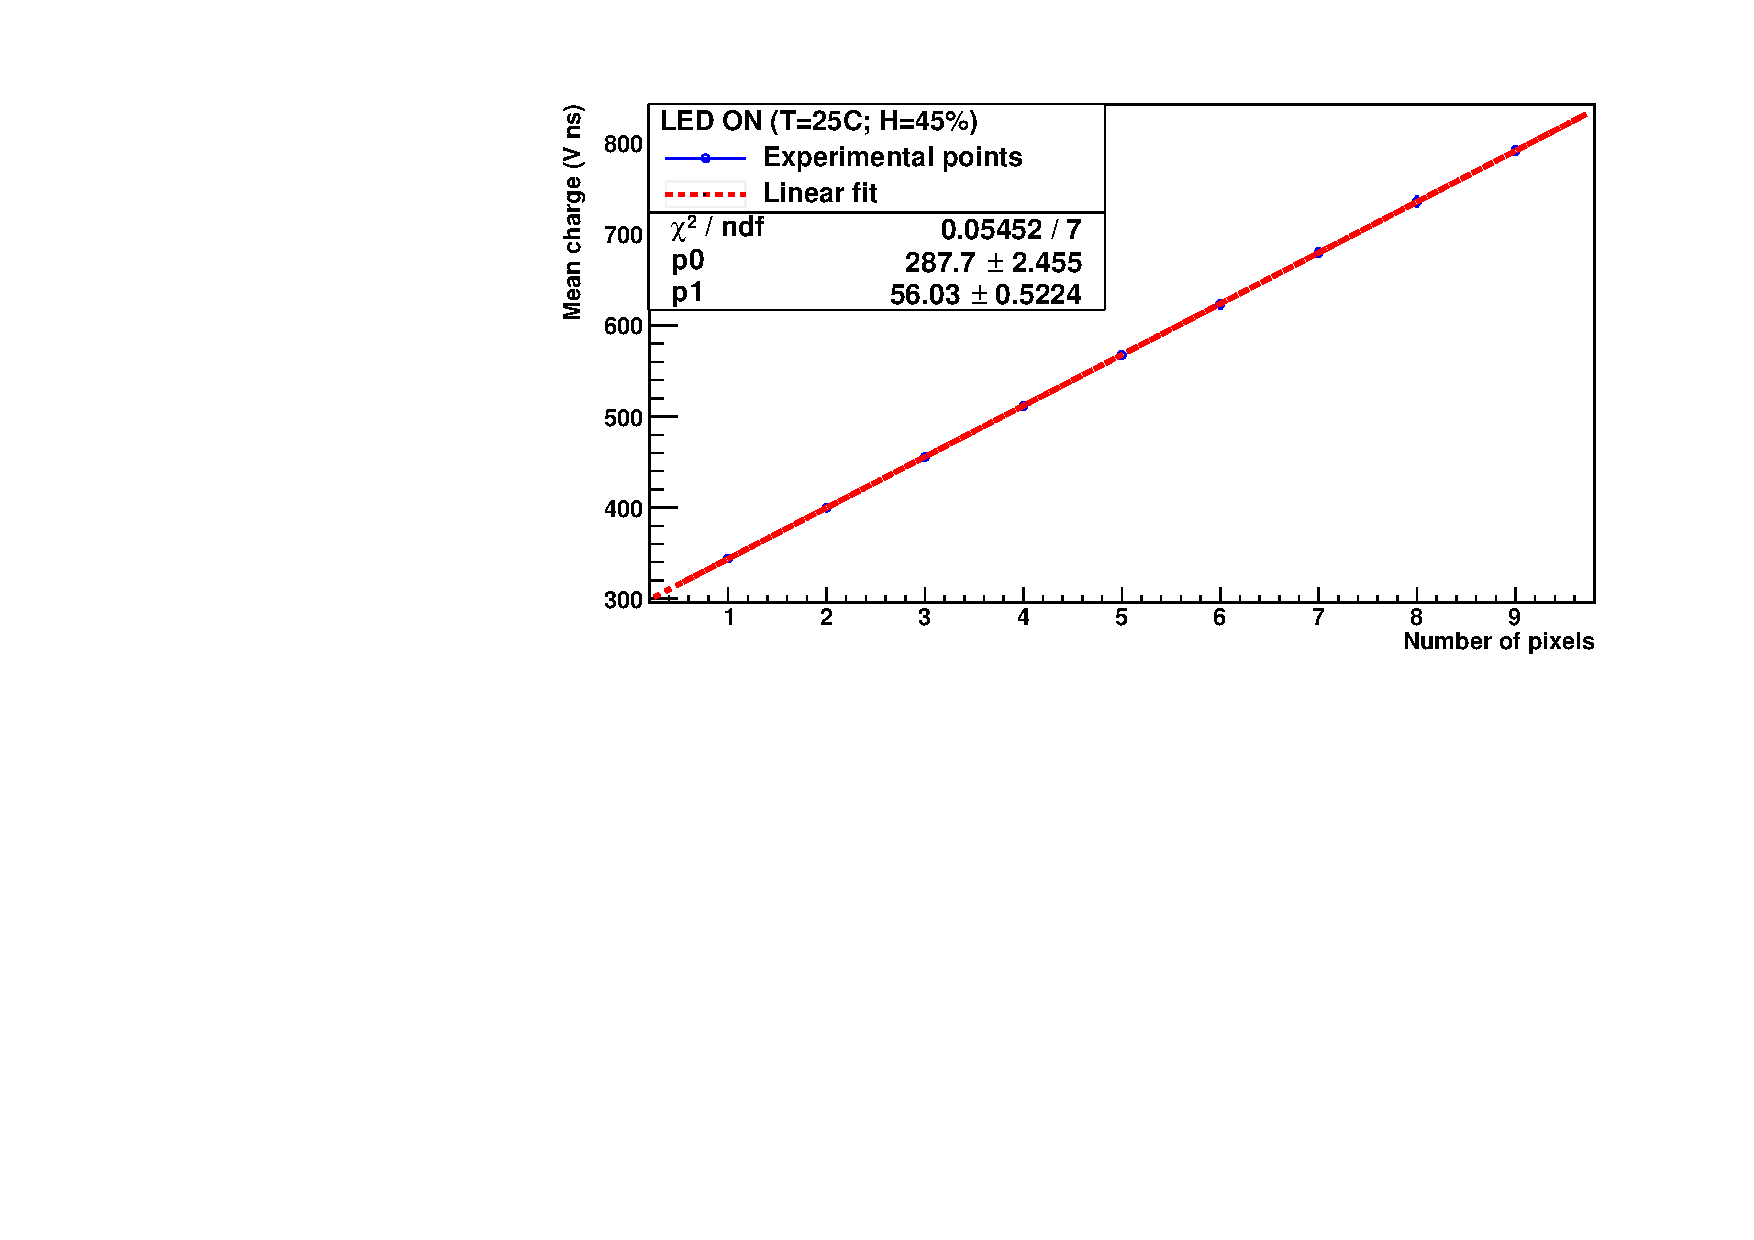
\includegraphics[width=\textwidth]{4ResearchAndDevelopments/42SiPM/LinearFit_Gain_NPixels.pdf}  
    \caption{\label{subfig:LinearFitSiPMGain}}
    \end{subfigure}
 \caption{ROOT analysis performed to obtian the SiPM gain. a) Fit of the SPS spectrum to various Gaussian functions. b) Charge of succesive number of pixels as a function of the number of pixels fired. Error bars are within point size. This experience was carried out at $T=25\celsius$, $V_{bias}=53.98~\volt$ and humidity of $H=45\%$.}
 \label{fig:ROOTAnalysisSiPMGain}
\end{figure}

%As can bee seen in Figure \ref{subfig:GaussianFitSiPMs}, a very good fit is achieved by the ROOT script with a $\chi^2$ test of $\frac{\chi^2}{ndf}=\frac{1276}{223}$. 

Up to 10 simultaneously fired pixels were obtained with a relative uncertainty of the charge measurement of less than $2\%$. The slope of the straight line in Figure \ref{subfig:LinearFitSiPMGain} corresponds to $\overline{\Delta Q}$.

The value obtained for the SiPM gain is $G_{SiPM}=4,11\cdot{} 10^{6}$, very close to the value provided by Hamamatsu, Table \ref{tab:PropertiesOfSiPM1375}.

A stabilization method for the SiPM gain was implemented. This is necessary for the TRITIUM project since the temperature in the final location of the tritium detector cannot be controlled with enough sensitivity to avoid variations of the SiPM gain. This method consists of compensating for variations in the SiPM gain caused by variations of temperature by controlled variations of the bias voltage. For this task, first, the dependence of the SiPM gain with the temperature and bias voltage was measured. The SiPM gain was measured at several temperatures from $15\celsius$ to $41\celsius$ in steps of $2\celsius$, which is expected to be the temperature range in the final location. The bias voltage was $V_{bias} = V_{BD}+3$. The SiPM gain was measured at several overvoltages from $1~\volt$ to $5~\volt$ in steps of $0.2~\volt$. The temperature was $T=25\celsius$. Both measurements are shown in Figure \ref{fig:SiPMGainDependance}. 

\begin{figure}
\centering
    \begin{subfigure}[b]{0.47\textwidth}
    \centering
    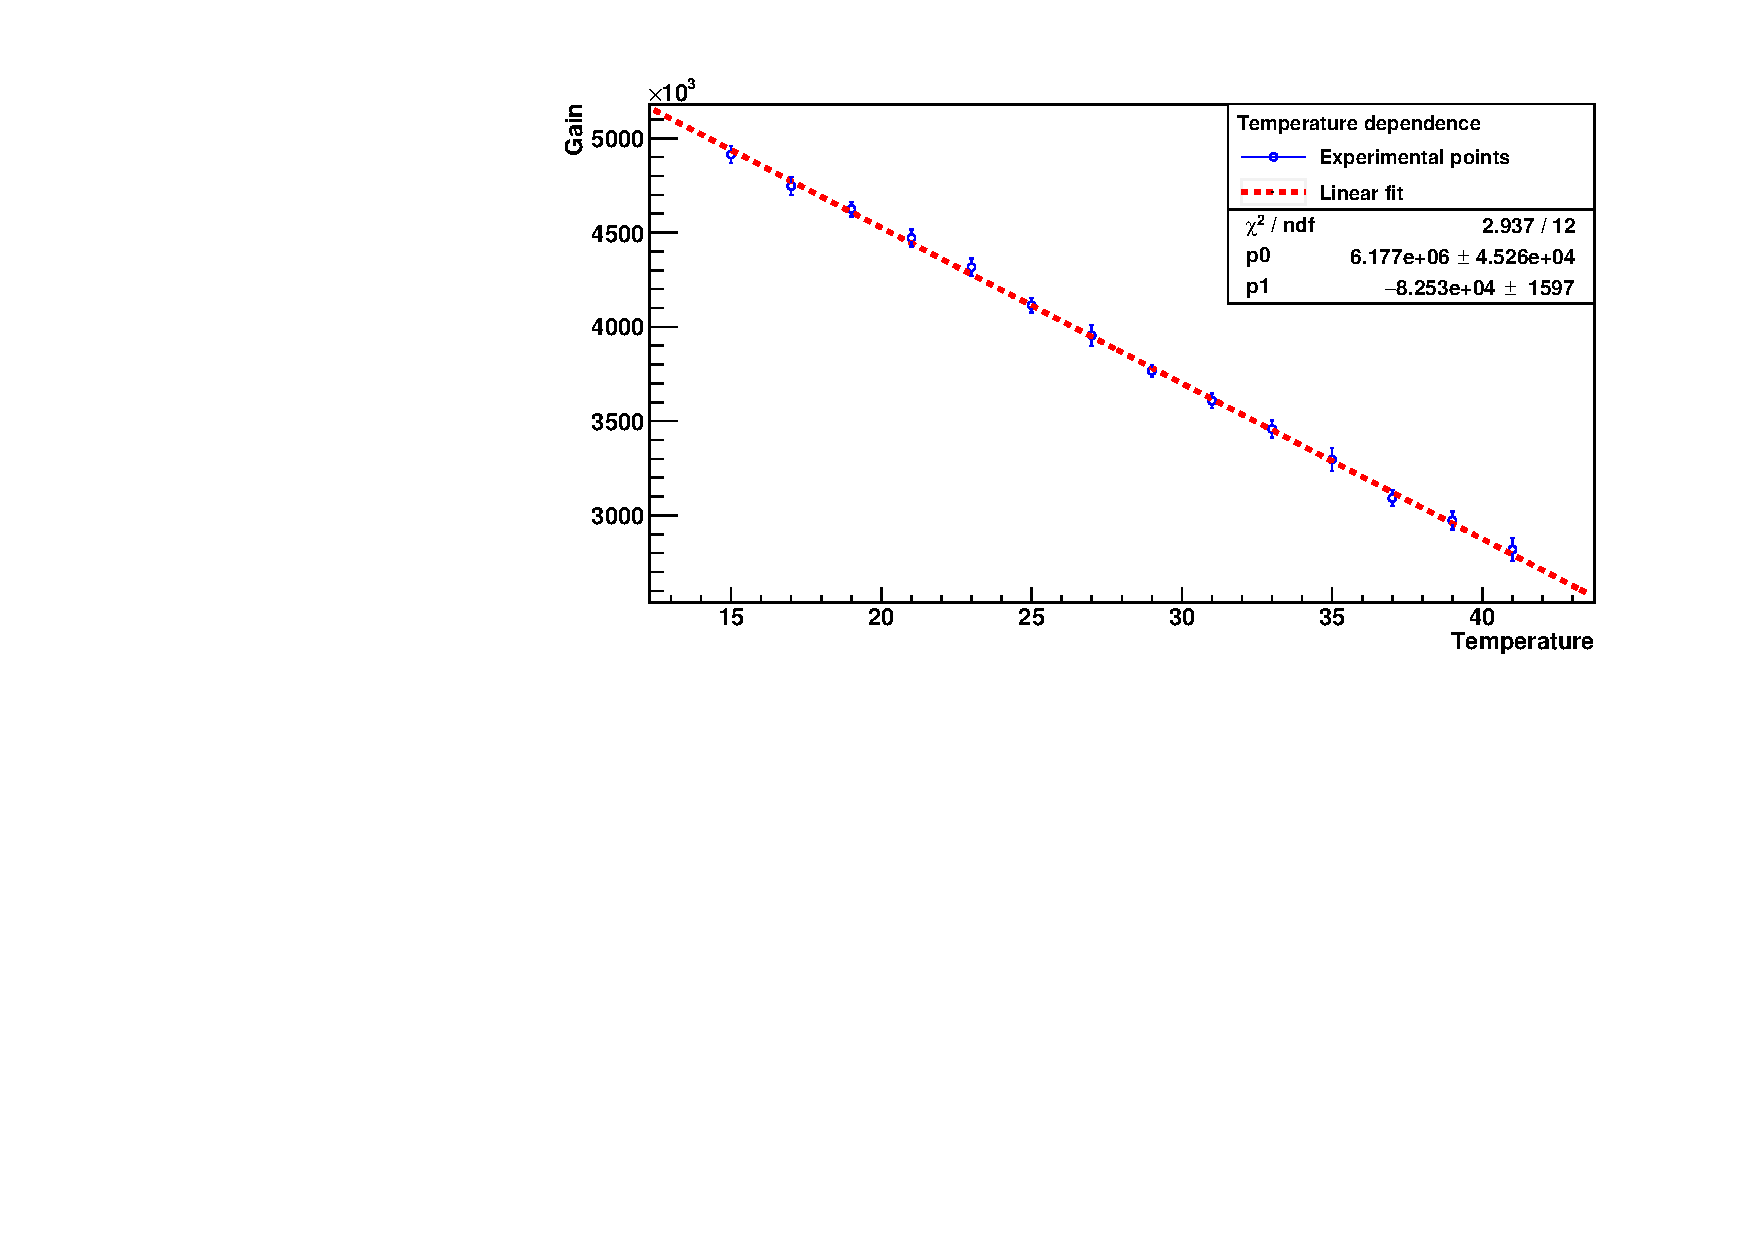
\includegraphics[width=\textwidth]{4ResearchAndDevelopments/42SiPM/SiPMGain_vs_Temperature.pdf}  
    \caption{\label{subfig:SiPMGainvsTemperature}}
    \end{subfigure}
    \hfill
    \begin{subfigure}[b]{0.47\textwidth}
    \centering
    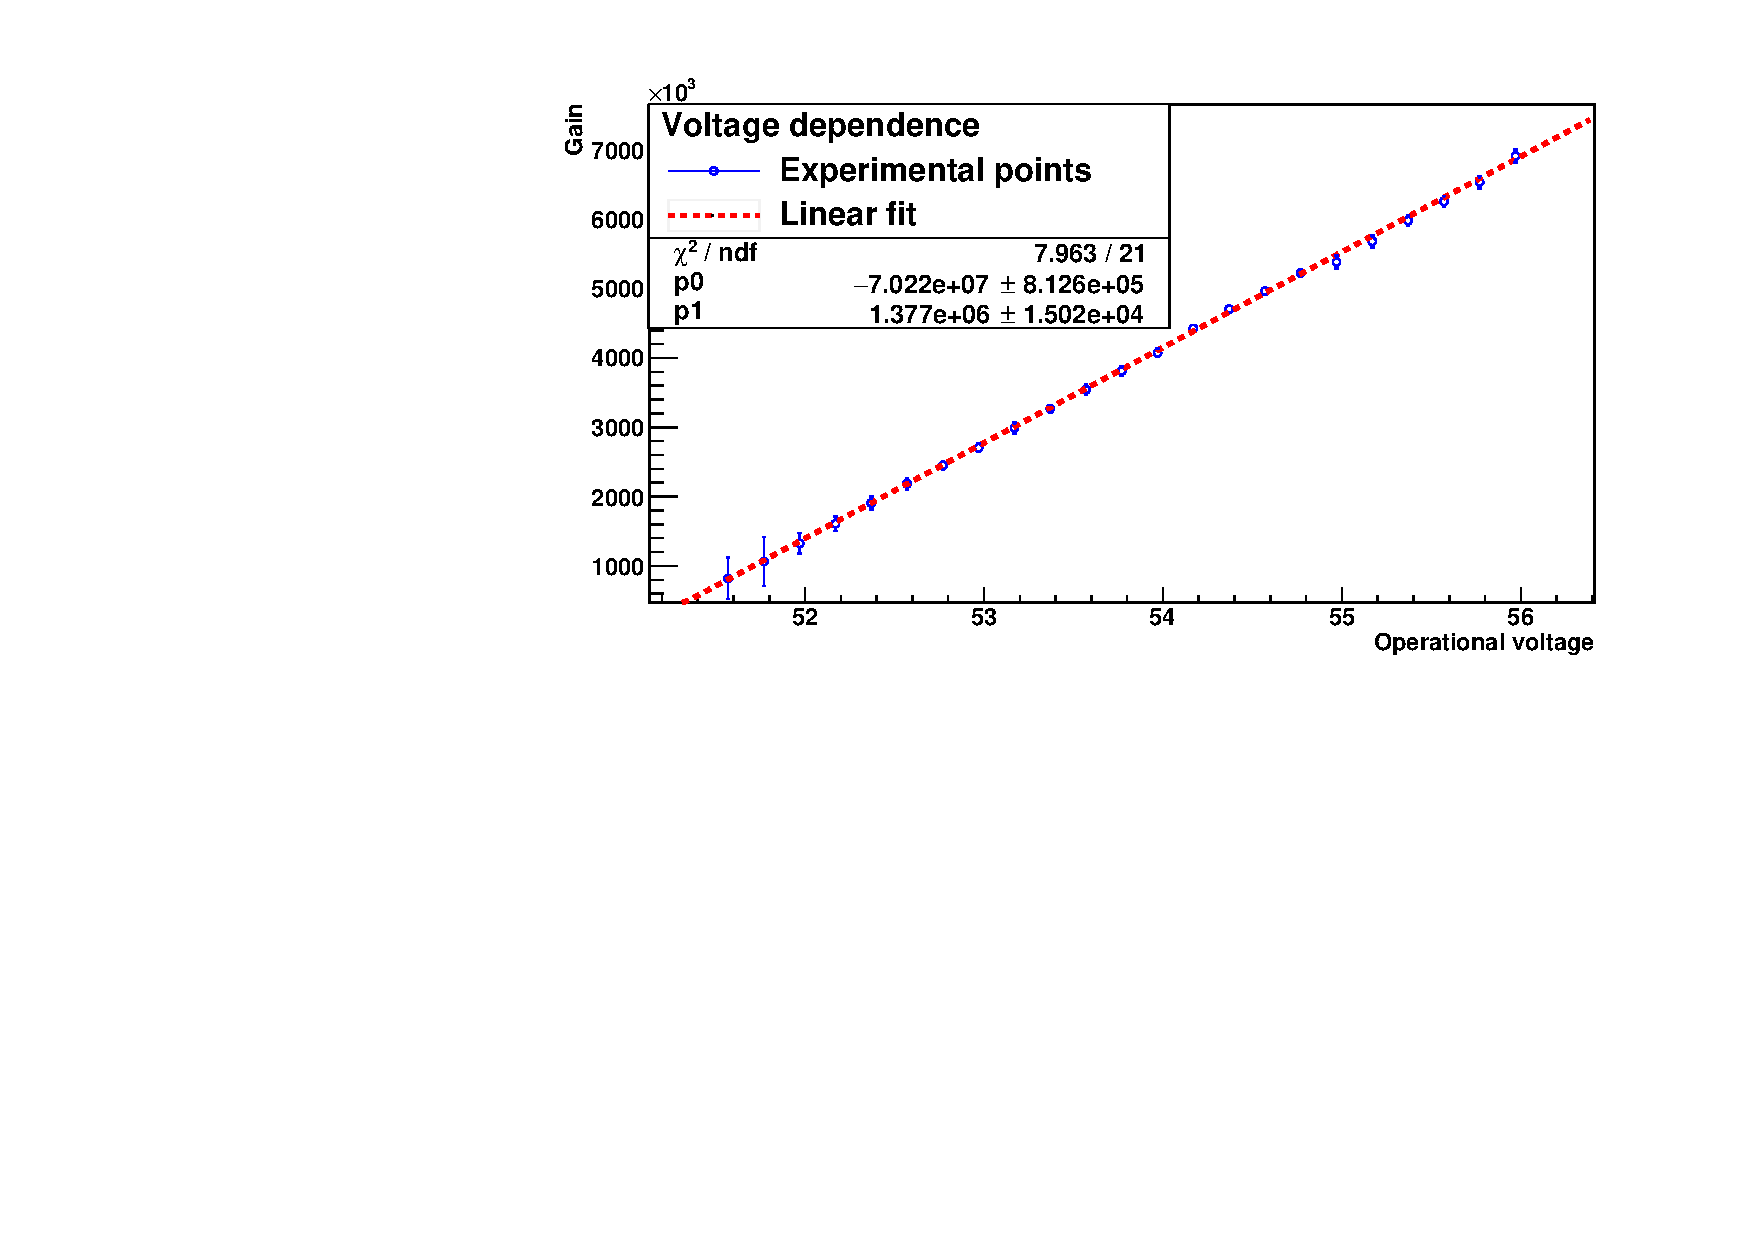
\includegraphics[width=\textwidth]{4ResearchAndDevelopments/42SiPM/SiPMGain_vs_Bias_Voltage.pdf}  
    \caption{\label{subfig:SiPMGainvsBiasVoltage}}
    \end{subfigure}
 \caption{Dependence of the SiPM gain with the a) Temperature b) Bias votlage.}
 \label{fig:SiPMGainDependance}
\end{figure}

As can be seen, an excellent linear trend is obtained for both cases. The  parameters of the linear fit obtained are,
\begin{equation*}
\begin{split}
G_{SiPM}=a \cdot{} T + b;& \qquad G_{SiPM}=c \cdot{} V_{bias} + d\\
a=\left( -82.53 \pm 1.59 \right) \cdot{} 10^{3};& \qquad c=\left( 137.72 \pm 1.50 \right) \cdot{} 10^{4}\\
b=\left( 617.65 \pm 4.53 \right) \cdot{} 10^{4};& \qquad d=\left( -762.16 \pm 8.13 \right) \cdot{} 10^{5} \\
\label{SiPMGainVSTempV}
\end{split}
\end{equation*} 

In addition, the breakdown voltage, $V_{BD}$, and the terminal capacitance, $C_t$, can be obtained from the linear fit of the SiPM gain as a function of the bias voltage, $V_{bias}$. Both parameters can be obtained from the definition of the SiPM gain and taking into account that the charge produced in a pixel is proportional to the capacitance of the pixel and the difference voltage in the SiPM, $V_{OV}$,
\begin{equation}
G_{SiPM}=\frac{Q_{pixel}}{e^-} = C_d \frac{V_{bias}-V_{BD}}{e^-} = c \cdot{} V_{bias}+d
\label{SiPMGain_Capacitance}
\end{equation}
where $C_d$ is the pixel capacitance.

From the linear fit obtained in Figure \ref{subfig:SiPMGainvsBiasVoltage}, a value of $V_{BD}=50.98 \pm 0.59~\volt$ and $C_d{}= 220.63 \pm 2.41~\text{f}\farad$ are obtained. The terminal capacitance of the SiPM can be calculated assuming all pixels in parallel, $C_{t}=N_{p}\times C_{d}=62.88 \pm 0.69~\pico\farad$. Both parameters, the breakdown voltage and the terminal capacitance, agree with the values provided by Hamamatsu, Table \ref{tab:PropertiesOfSiPM1375}. 

Finally, the value of the bias voltage to be applied to compensate for the variation in the SiPM gain due to a variation of the temperature can be obtained by applying variations to linear relations:
\begin{equation*}
\begin{split}
G_{SiPM}=a \cdot{} T + b  &\longrightarrow \partial G_{SiPM}= a \partial T\\
G_{SiPM}=c \cdot{} V_{bias} + d &\longrightarrow \partial G_{SiPM}= c \partial V_{bias}
\label{Gain_compensationVariations}
\end{split}
\end{equation*} 
Therefore, the total variation of the SiPM gain, which is produced by the variation of both parameters, must be cancel:
\begin{equation*}
\begin{split}
\partial G_{SiPM, tot}= \partial G_{SiPM}(T) &+ \partial G_{SiPM}(V_{bias}) = 0\\ 
\partial G_{SiPM}(V_{bias}) = -\partial G_{SiPM}(T) &\longrightarrow c \partial V_{bias} = - a \partial T\\ 
\partial V_{bias}  = - \frac{a}{c}&\partial T = e \partial T
\label{Gain_compensation0}
\end{split}
\end{equation*} 
where the parámeter $e= 59.93 \pm 1.33~\milli\volt/\celsius $ is the ratio of $a$ and $c$ and agrees with the value of the temperature coeficient provided by Hamamtsu, Table \ref{tab:PropertiesOfSiPM1375}. Finally, integrating this expression, we obtain:
\begin{equation}
\begin{split}
\int_{V_i}^{V_f}\partial V_{bias}  = e\int_{T_i}^{T_f}\partial T \longrightarrow \Delta V_{bias} = e \Delta T
\label{Gain_compensationIntegring}
\end{split}
\end{equation} 
This equation gives the variation of the voltage, $\Delta V_{bias}$, that keeps the SiPM gain when there is a variation, $\Delta T$, of the temperature. More relevant is to know the bias voltage, $V_{bias}$ to be applied as a function of the temperature, $T$. For this, it is necessary a reference situation. In our case, the reference situation considered is $V_i=V_{ref}= V_{BD}+3~\volt = 53.98~\volt$ and $T_i=T_{ref}=24\celsius$, at which the gain is $4.2 \cdot{} 10^{6}$ (experimentally measured). Thus, we get:
\begin{equation*}
\begin{split}
(V_{bias}-V_{ref} )= e \left( T -T_{ref} \right) 
\label{Gain_compensationEquation}
\end{split}
\end{equation*}
\begin{equation}
V_{bias}(\volt)= 59.9 \cdot{} 10^{-3} \cdot{} T(\celsius) + 52.54
\label{Gain_compensationReference}
\end{equation}  
Finally, the stabilization method of the SiPM gain developed was tested. The temperature was varied from $21\celsius$ to $29\celsius$ and the bias voltage was modified according to the equation \ref{Gain_compensationReference}. The value of the SiPM gain obtained is shown in Figure \ref{fig:SiPMGainStabilization} as a function of the temperature.

\begin{figure}[hbtp]
\centering
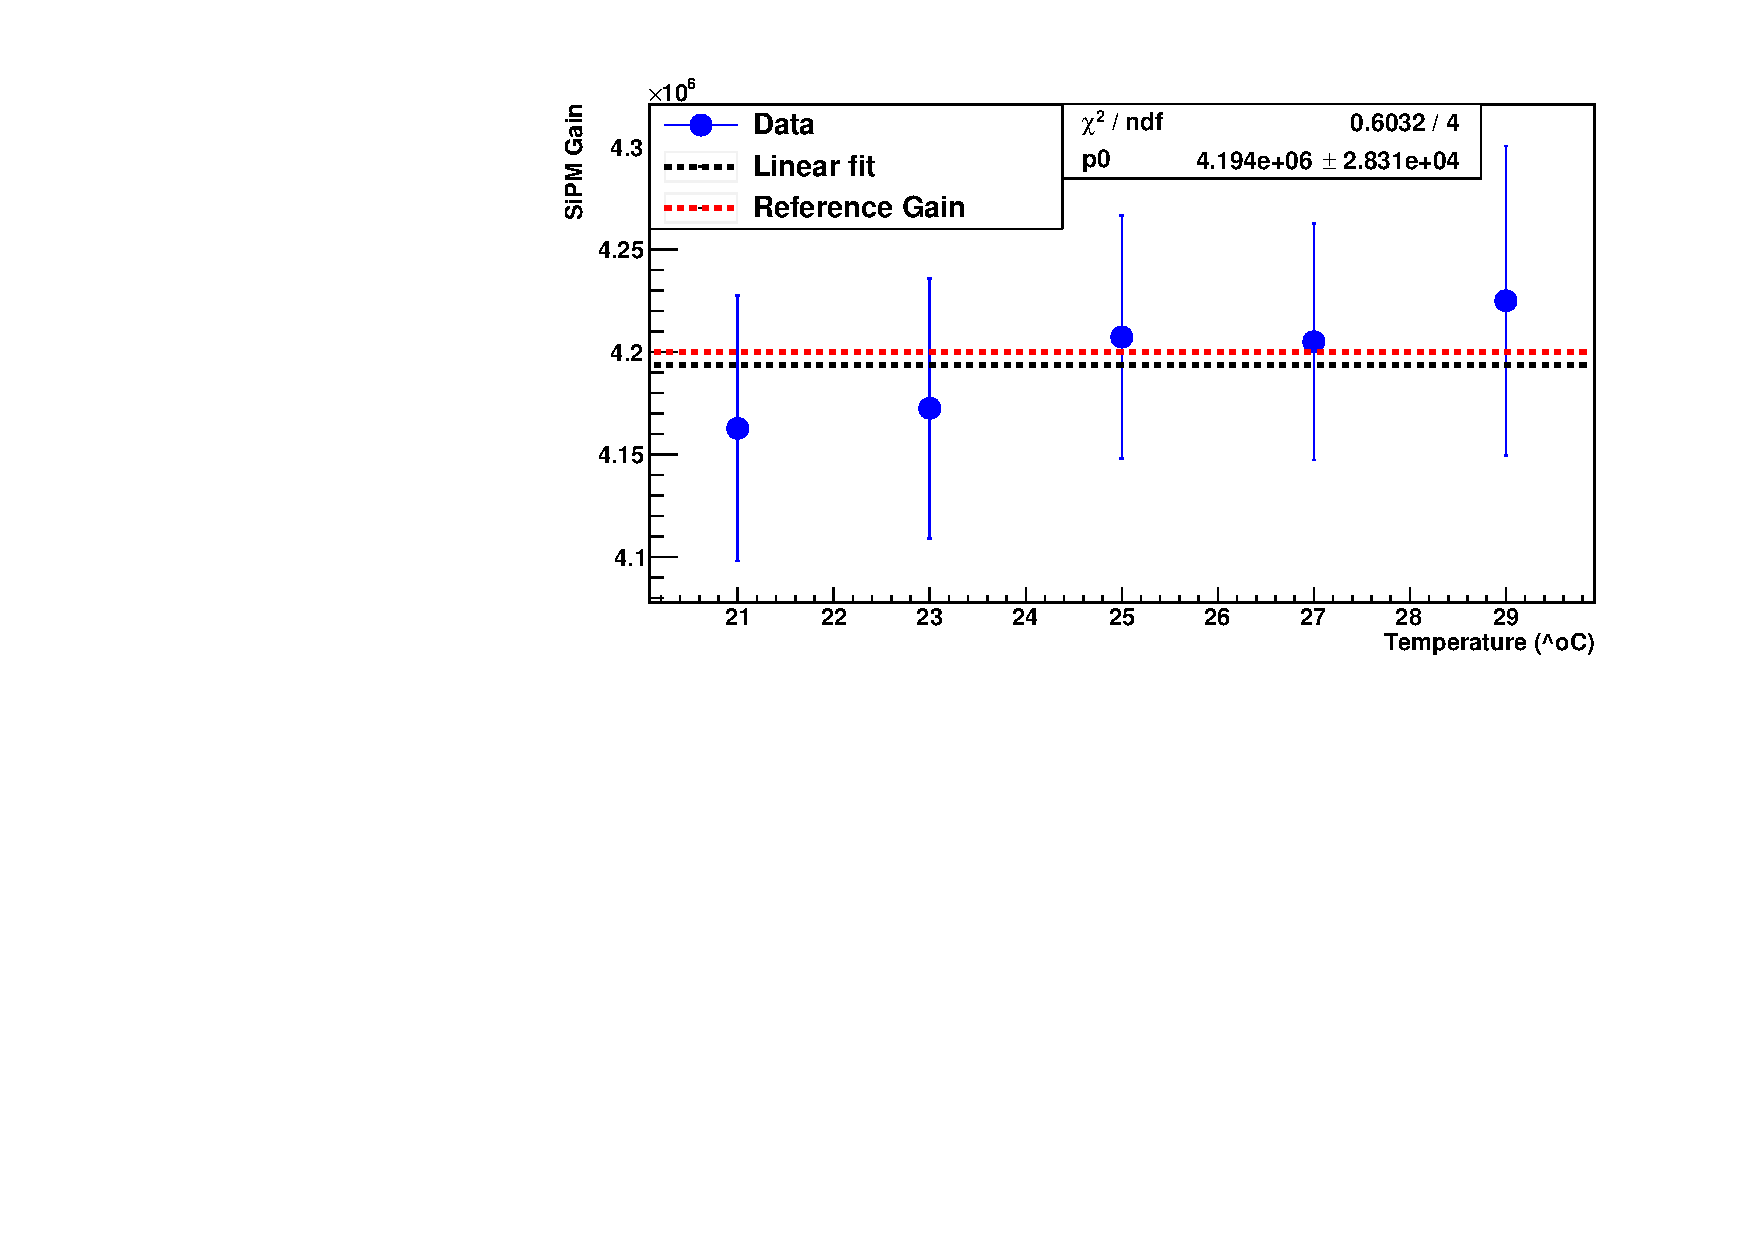
\includegraphics[scale=0.6]{4ResearchAndDevelopments/42SiPM/SiPMGain_Stabilization.pdf}
\caption{SiPM gain as a function of the temperature with the stabilization method. \label{fig:SiPMGainStabilization}}
\end{figure}

A red dotted line is included, indicating the value of the SiPM gain to be kept. The SiPM gain is maintained fairly well by this method.